\begin{figure}[h]
    \centering
    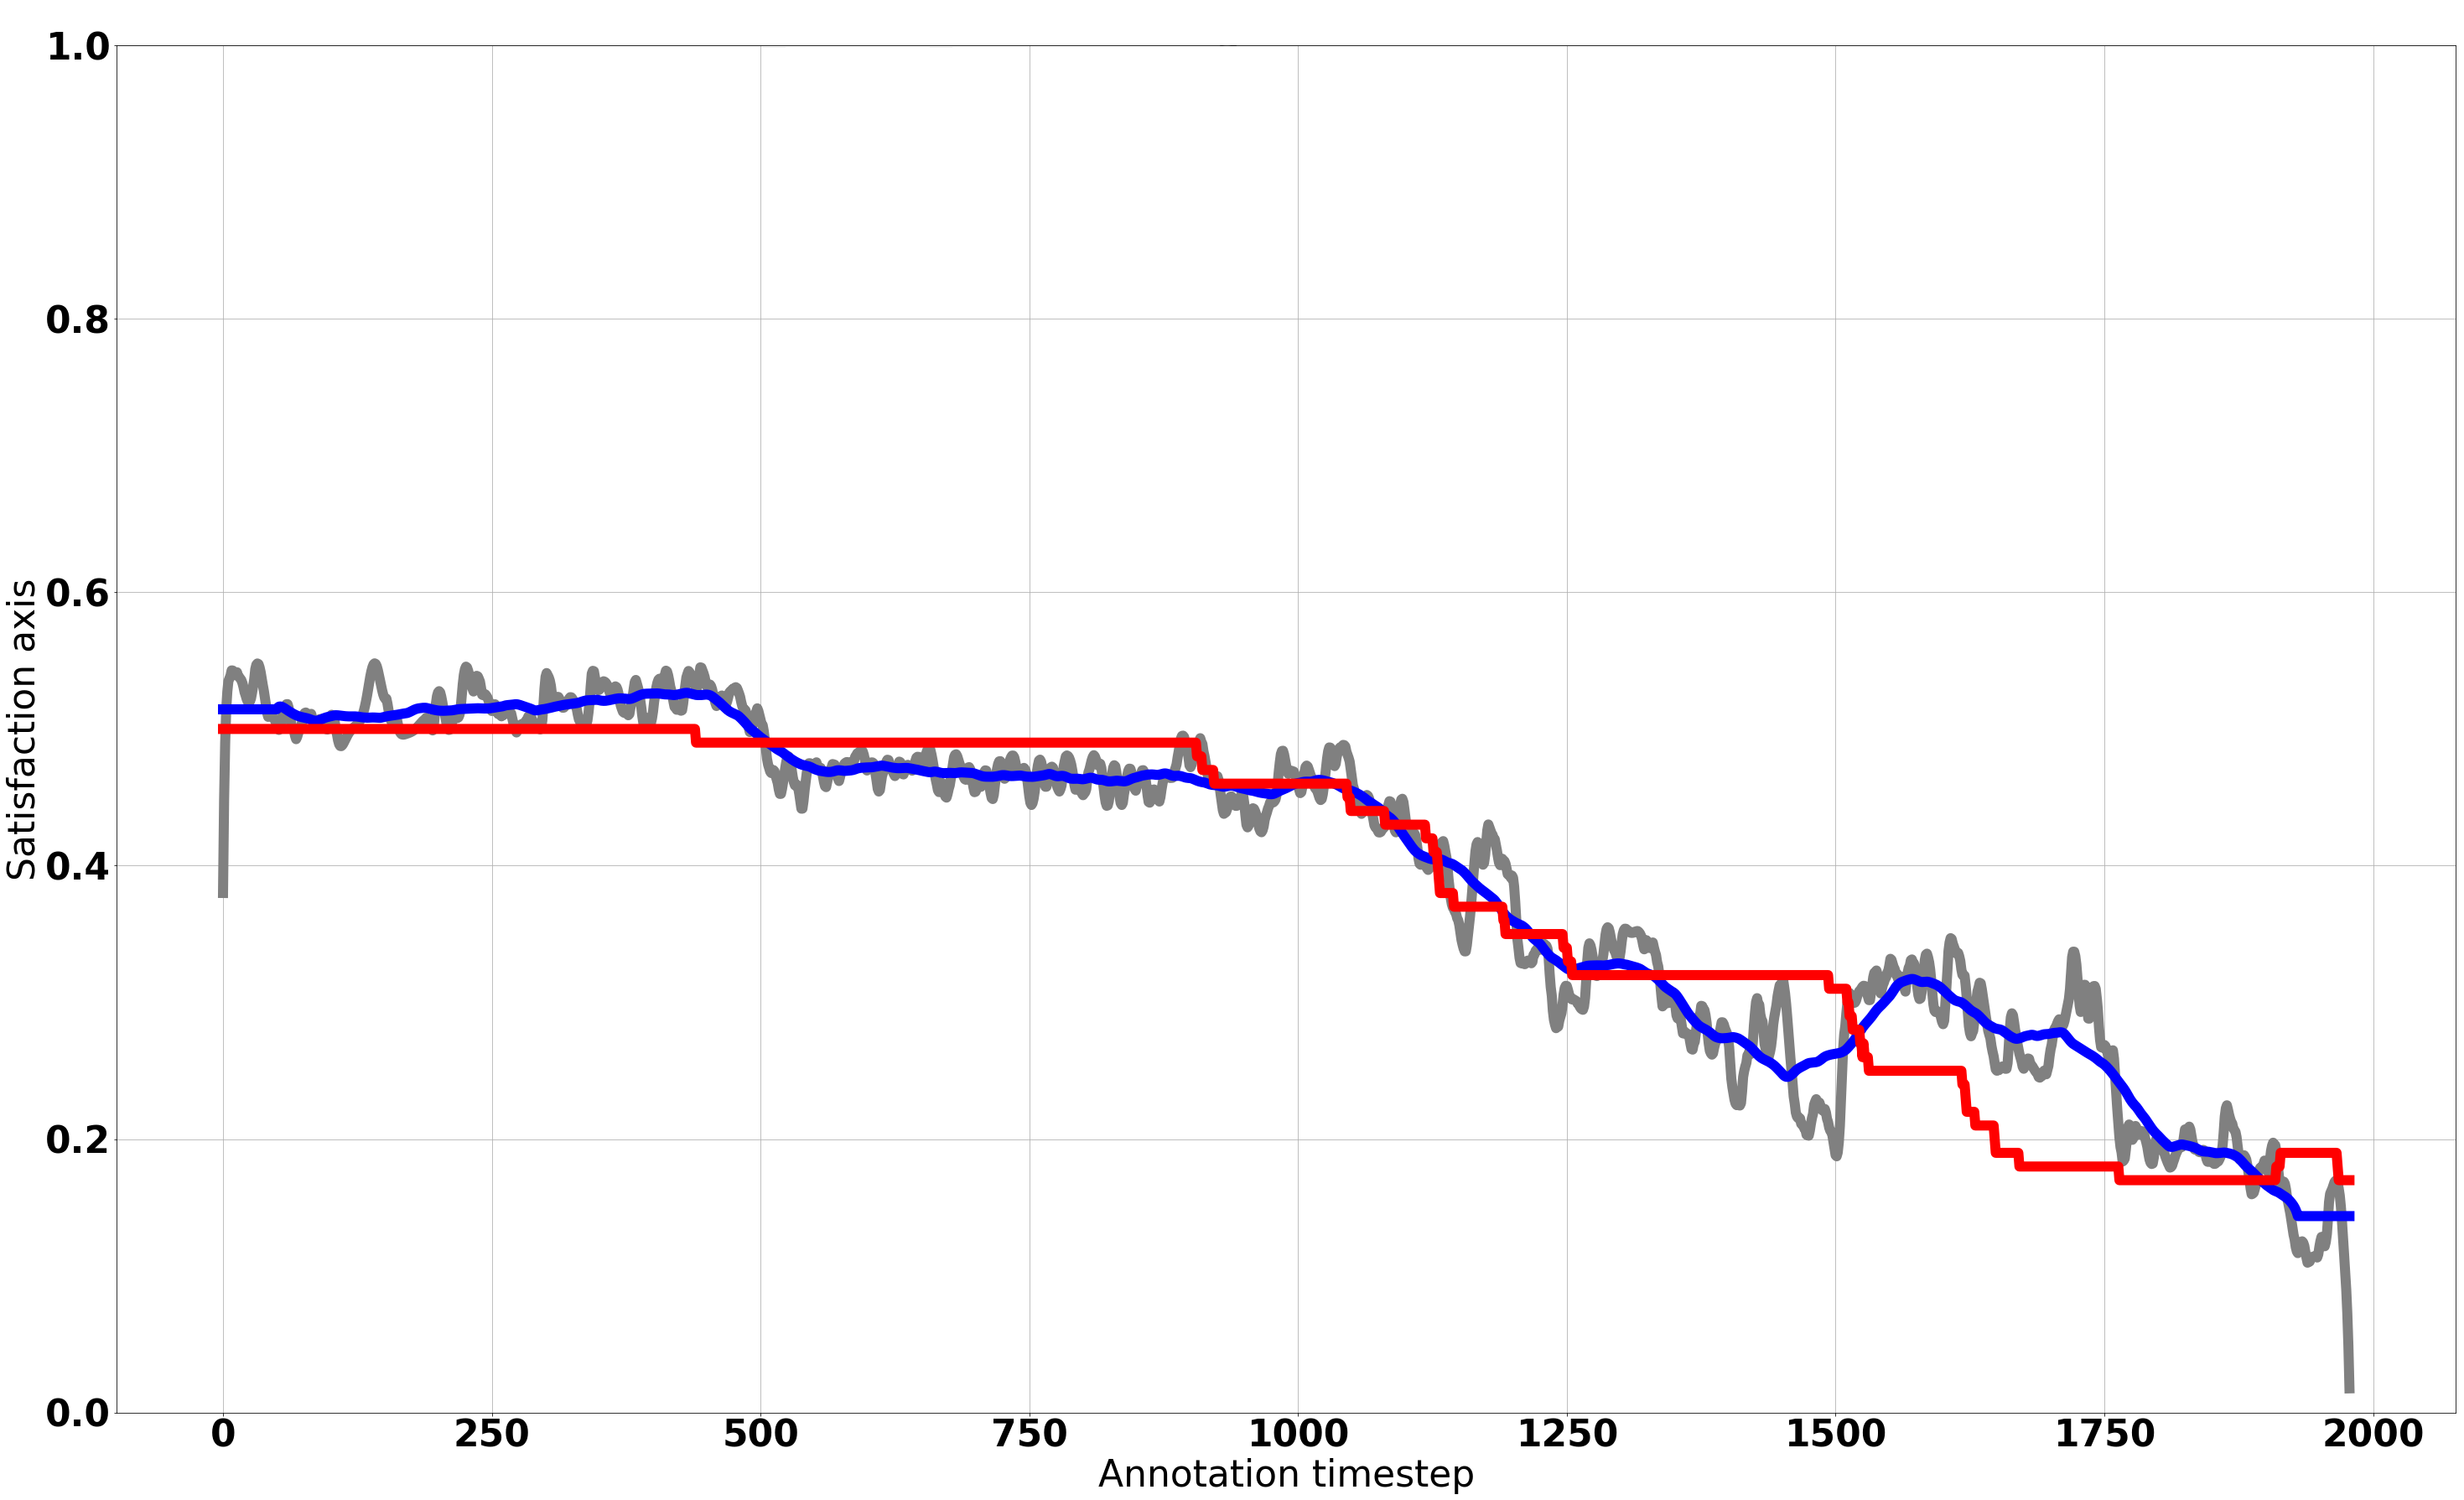
\includegraphics[width=.99\linewidth]{./Chapitre5/figures/lissage2.png}
    % \begin{subfigure}{.49\textwidth}
    %   \centering
    %   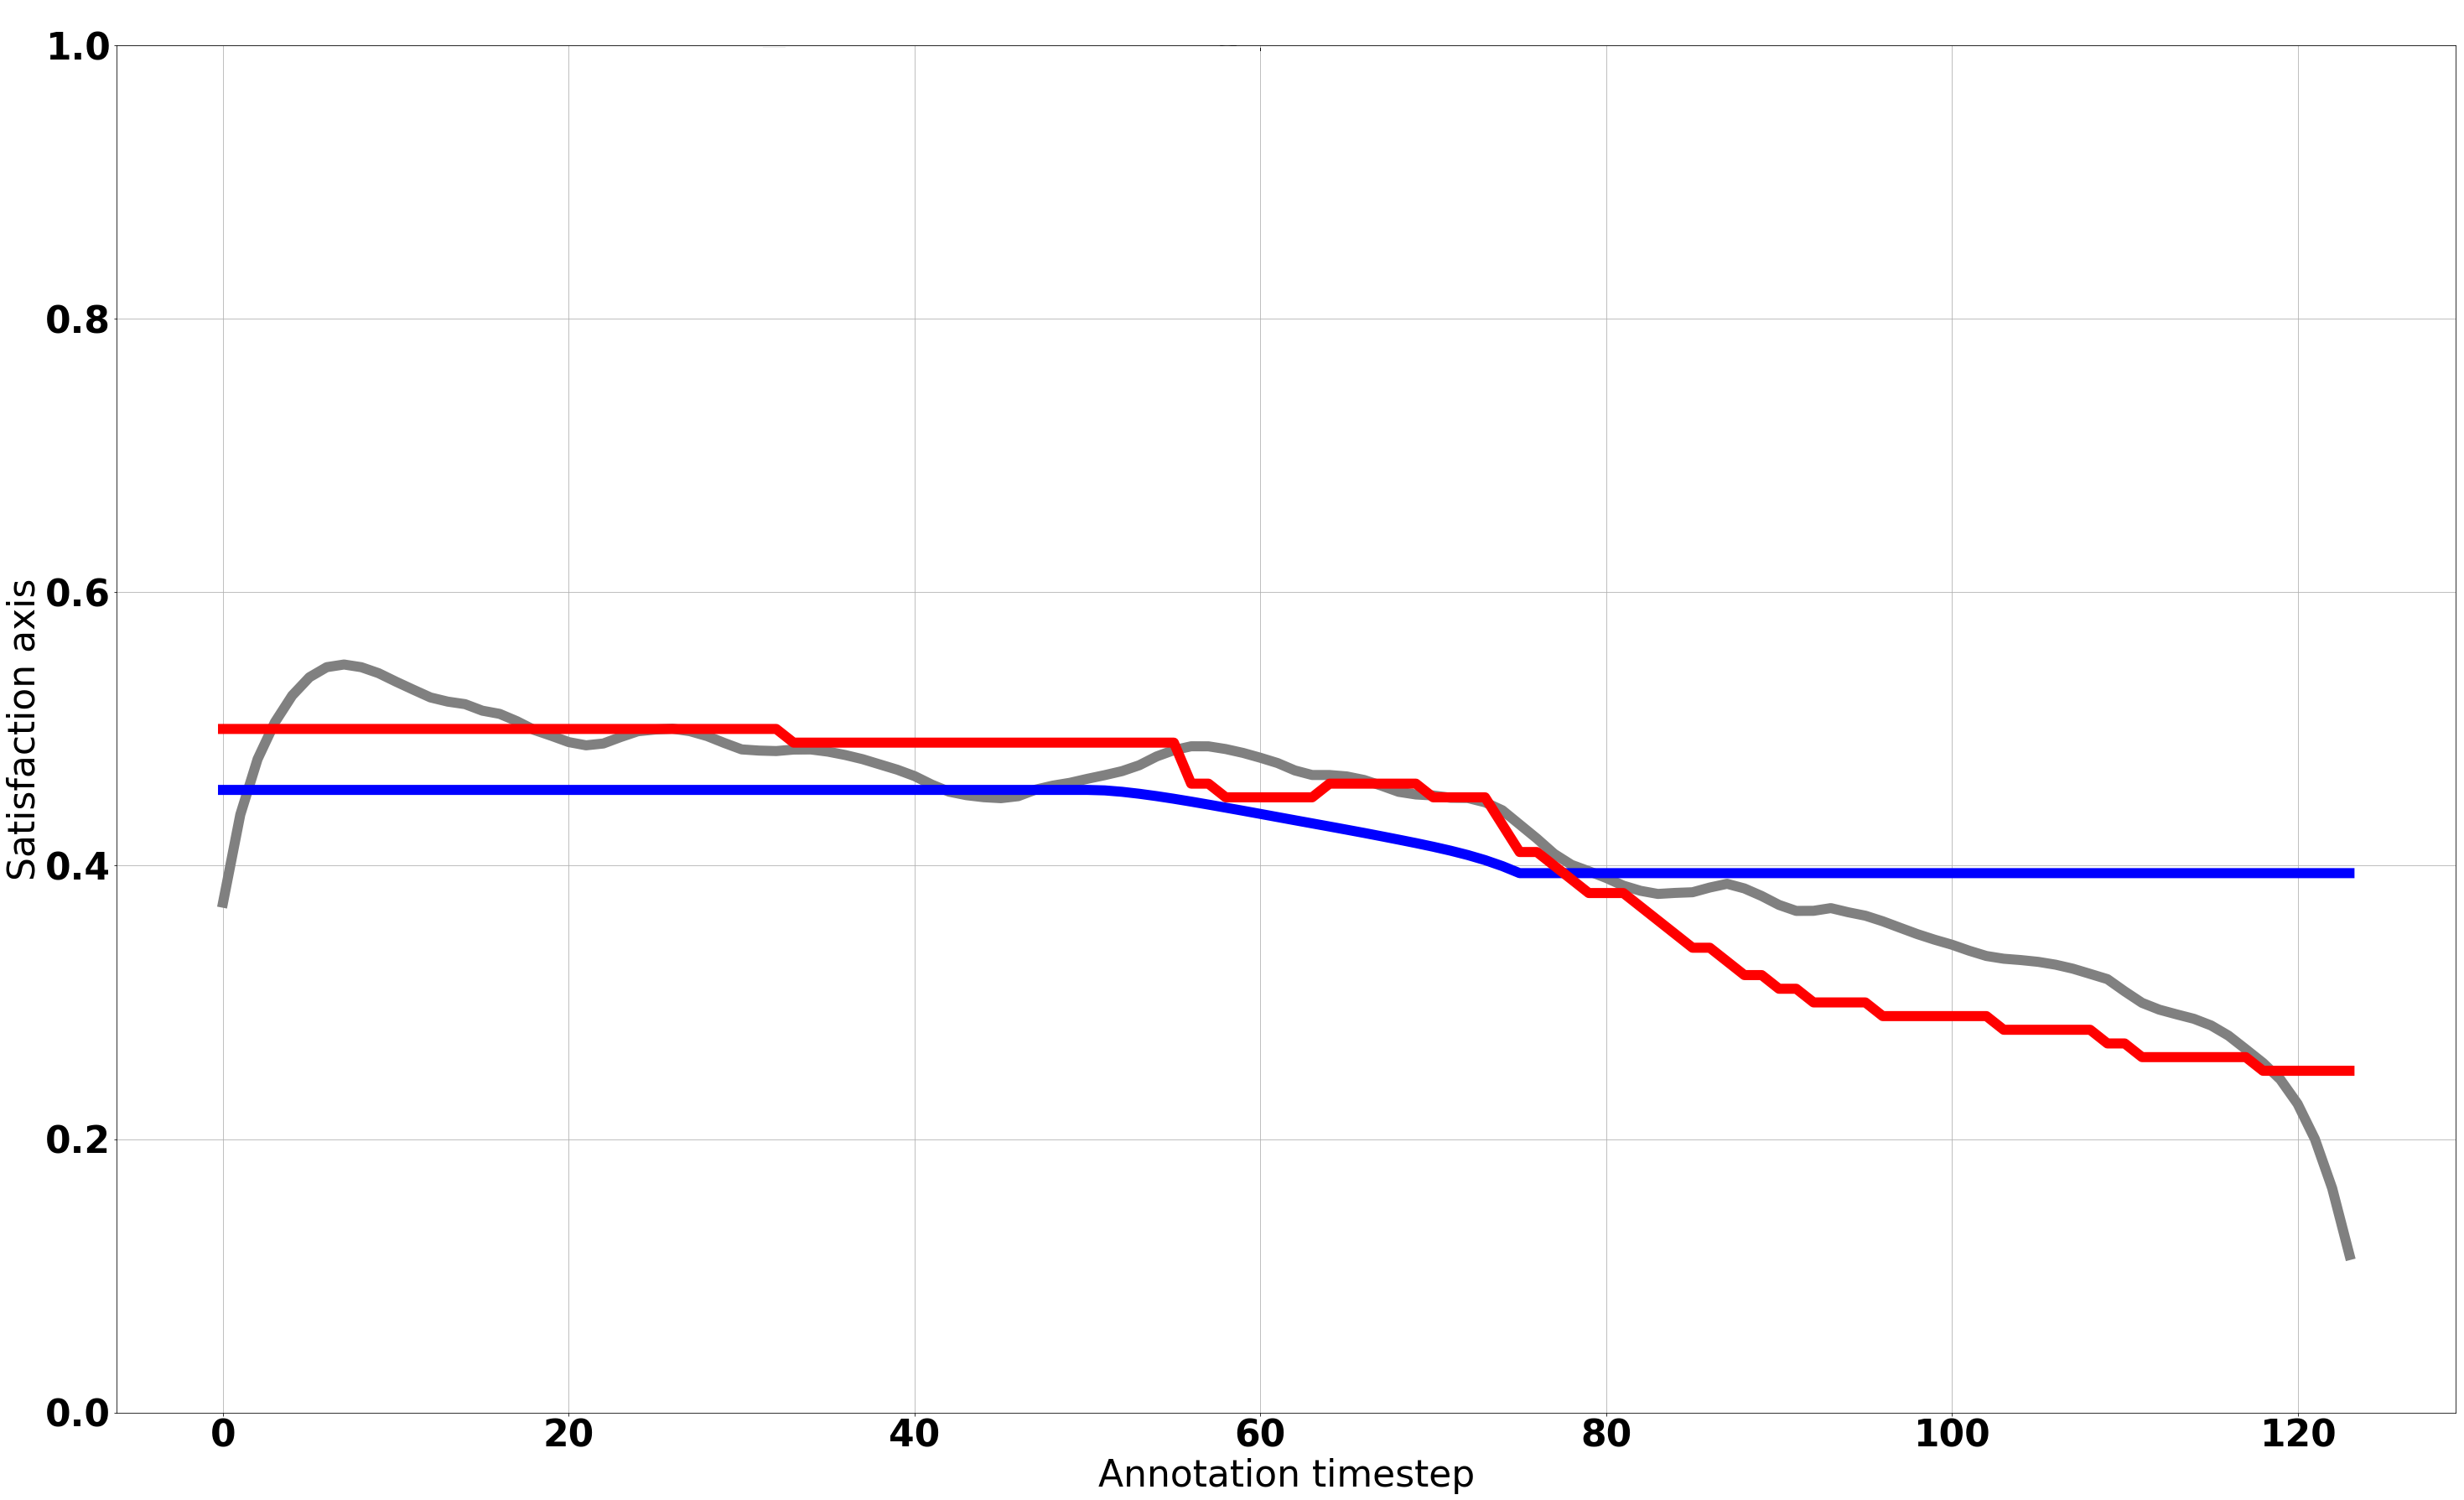
\includegraphics[width=.99\linewidth]{./Chapitre5/figures/lissage1.png}
    % \end{subfigure}
    % \begin{subfigure}{.49\textwidth}
    %   \centering
    %   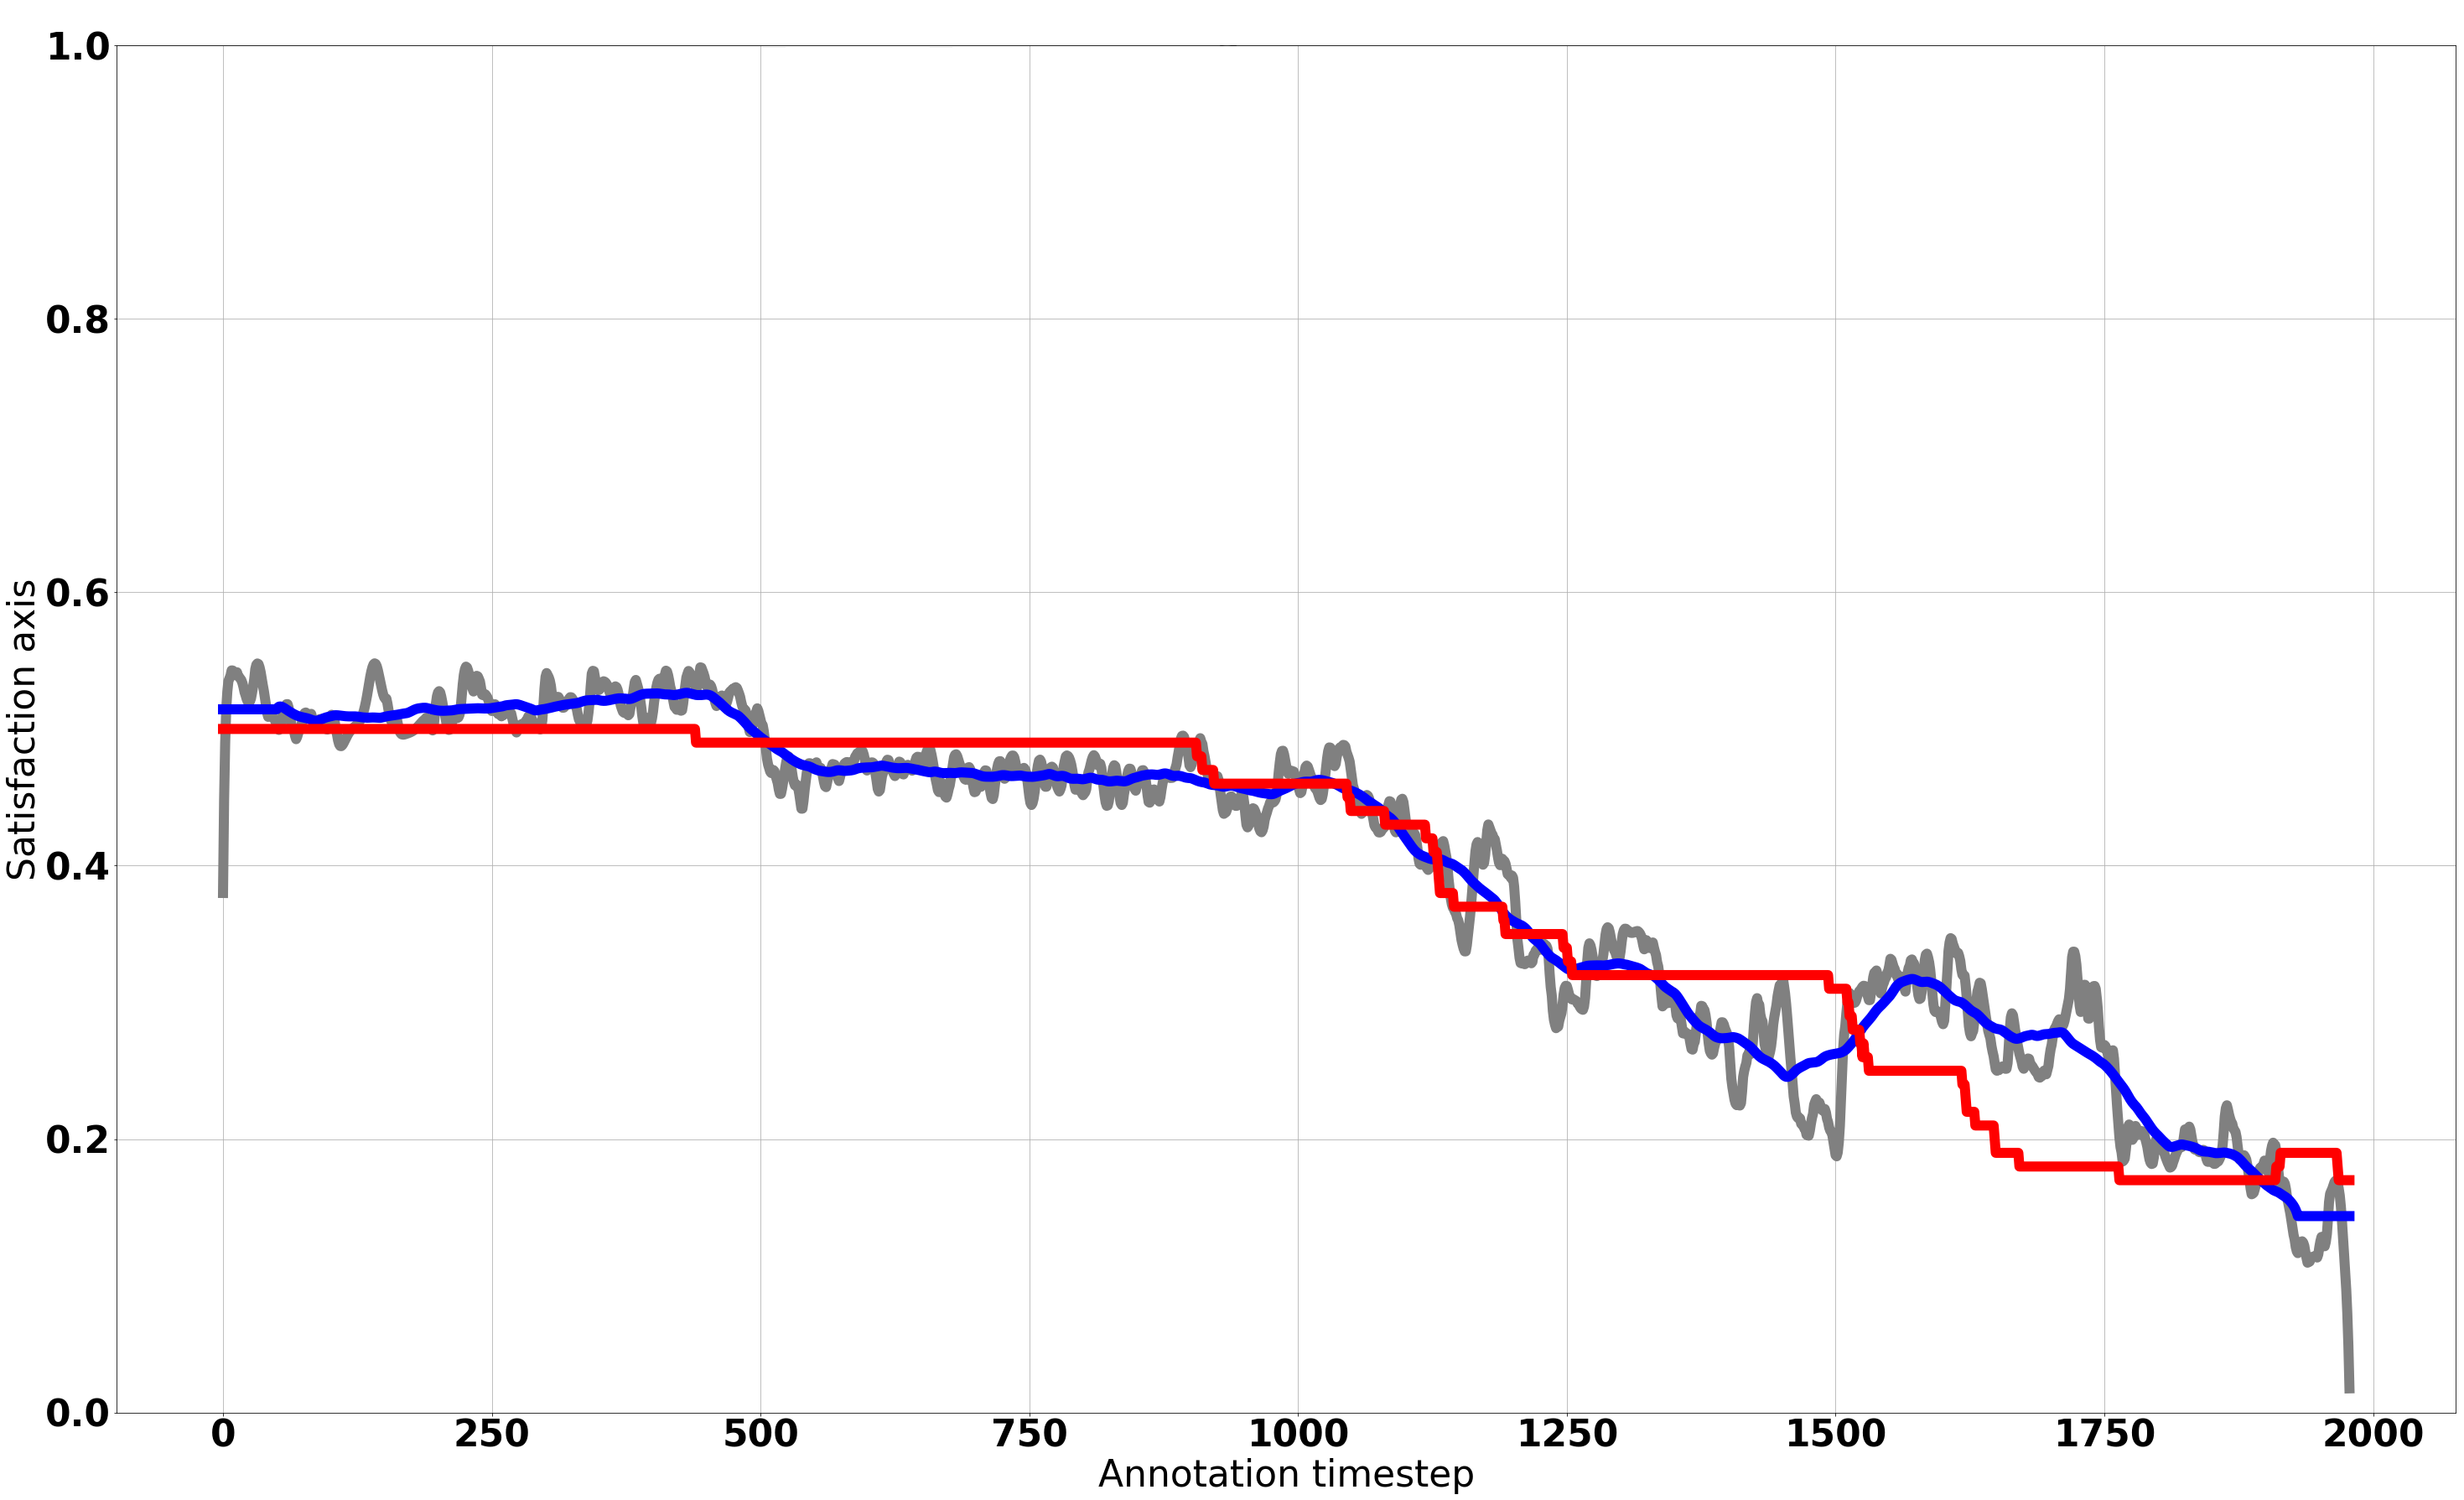
\includegraphics[width=.99\linewidth]{./Chapitre5/figures/lissage2.png}
    % \end{subfigure}
    \caption{Comparaison entre les prédictions lissées et non lissées d'une conversation de l'ensemble de test d'AlloSat. La référence est en rouge, les prédictions en gris et les prédictions lissés en bleu.}
    \label{fig:lissage}
\end{figure}
